El algoritmo de detección de tubos implementa una secuencia de cuatro etapas que progresivamente extraen y refinan información estructural hasta identificar el tubo objetivo.\\

\underline{Etapa 1 - Detección de bordes mediante Canny}: Se aplica el algoritmo de Canny sobre la imagen convertida a escala de grises. Se aplica filtrado gaussiano ($5 \times 5$ píxeles), cálculo de gradientes mediante Sobel, supresión de no-máximos y doble umbralización con histéresis ($T_{bajo} = 20$, $T_{alto} = 172$). El resultado es una imagen binaria con los bordes del tubo y elementos de cultivo.\\

\underline{Etapa 2 - Filtrado por canal de saturación}: Para discriminar bordes del fondo, se explota que el PVC blanco presenta baja saturación. Se extrae el canal S del espacio HSV, se invierte ($S_{inv} = 255 - S$) y se umbraliza ($T_S = 150$). Los bordes de Canny se filtran mediante AND binario con esta máscara.\\

\underline{Etapa 3 - Refinamiento morfológico}: Para conectar segmentos de borde fragmentados por discontinuidades, se aplica cierre morfológico con elemento estructurante rectangular de $3 \times 9$ píxeles. La orientación vertical del kernel favorece la conexión de líneas horizontales (bordes del tubo) mientras preserva la separación entre líneas verticales.


\underline{Etapa 4 - Detección de contornos y scoring}: Se ejecuta el algoritmo de Suzuki-Abe filtrando contornos por área mínima de 250 píxeles. Se calcula la relación de aspecto $AR = w/h$ y se descartan contornos con $AR \geq 0.9$ (elementos horizontales). Los contornos verticales se evalúan mediante scoring que combina: relación de aspecto (favorece $AR < 0.5$), área normalizada (favorece tamaños intermedios) y homogeneidad de saturación (favorece color uniforme). El contorno con mayor puntuación se selecciona como tubo objetivo.

\begin{figure}[H]
\centering
\begin{subfigure}[b]{0.48\textwidth}
    \centering
    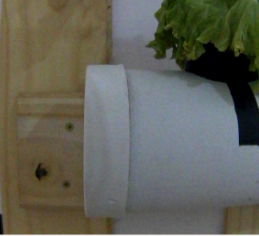
\includegraphics[width=0.7\textwidth]{imagenes/detector_tubos_1_original.png}
    \caption{Imagen RGB original}
\end{subfigure}
\hfill
\begin{subfigure}[b]{0.48\textwidth}
    \centering
    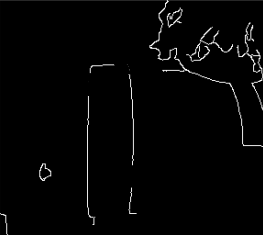
\includegraphics[width=0.7\textwidth]{imagenes/detector_tubos_2_canny.png}
    \caption{Bordes Canny (T=20-172)}
\end{subfigure}

\vspace{0.3cm}

\begin{subfigure}[b]{0.48\textwidth}
    \centering
    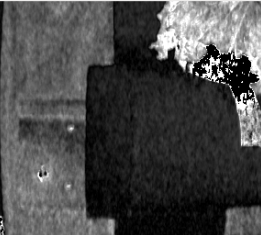
\includegraphics[width=0.7\textwidth]{imagenes/detector_tubos_3_canal_s.png}
    \caption{Máscara de baja saturación}
\end{subfigure}
\hfill
\begin{subfigure}[b]{0.48\textwidth}
    \centering
    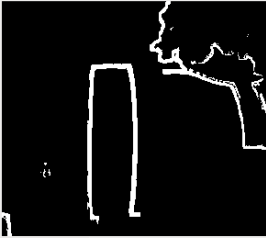
\includegraphics[width=0.7\textwidth]{imagenes/detector_tubos_5_morfologia.png}
    \caption{Morfología de cierre (kernel 3×9)}
\end{subfigure}

\vspace{0.3cm}

\caption{\textit{Procesamiento del detector de tubos mostrando las transformaciones sucesivas hasta la identificación de bordes del tubo}}
\label{fig:proceso_tubos}
\end{figure}

El algoritmo implementa mecanismos de validación ante casos ambiguos. Sin contornos válidos, retorna valores nulos indicando ausencia de tubo. Con múltiples candidatos similares selecciona el de mayor score. 

\begin{figure}[H]
    \centering
    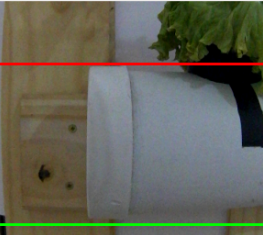
\includegraphics[width=0.4\textwidth]{imagenes/detector_tubos_6_lineas.png}
    \caption{\textit{Líneas superior e inferior detectadas}}
    \label{fig:detector_tubos_lineas}
\end{figure}

\subsubsection{Métricas de desempeño}
Evaluado sobre 28 frames de barrido vertical (14 con tubos, 14 sin tubos):

\begin{table}[H]
\centering
\begin{tabular}{|l|r|}
\hline
\textbf{Métrica} & \textbf{Valor} \\ \hline
Sensibilidad (Recall) & 92.9\% (13/14) \\ \hline
Especificidad & 100\% (14/14) \\ \hline
Precisión (Precision) & 100\% (13/13) \\ \hline
Error de localización Y medio & 4.7 mm \\ \hline
Error máximo de localización Y & 12.3 mm \\ \hline
\end{tabular}
\caption{Desempeño del detector de tubos}
\label{tab:metricas_tubos}
\end{table}

Matriz de detección para tubos:

\begin{table}[H]
\centering
\begin{tabular}{cc|c|c|}
\cline{3-4}
& & \multicolumn{2}{c|}{\textbf{Predicción}} \\ \cline{3-4}
& & Tubo detectado & No tubo \\ \hline
\multicolumn{1}{|c|}{\multirow{2}{*}{\textbf{Real}}} & Tubo & 13 & 1 \\ \cline{2-4}
\multicolumn{1}{|c|}{} & No tubo & 0 & 14 \\ \hline
\end{tabular}
\caption{Matriz de detección binaria - tubos}
\label{tab:confusion_tubos}
\end{table}

\noindent
El único falso negativo se debió a reflejo especular que saturó el canal V del sensor.
